
\subsection{VALUATION APPROACHES}

In practice, there are three generally accepted valuation approaches to estimate the fair value of an ongoing business, investment project, and its tangible and intangible assets. These approaches are briefly described below:

\begin{figure}[H]
\centering
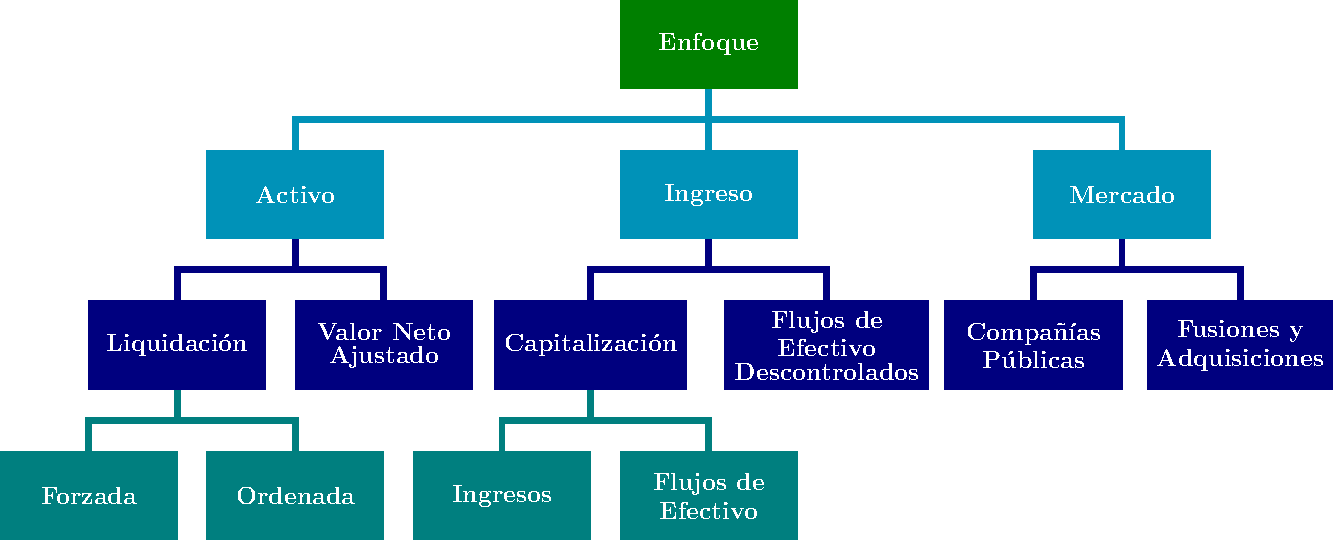
\includegraphics[width=14cm]{\rutaImagenes/enfoques_mas_utilizados_eng}
\end{figure}

\subsubsection{Asset Approach}

The asset approach is a general way to determine the fair value of a company's equity, a business, investment project, tangible asset, or intangible asset using one or more methods based on the value of assets and their net liabilities.\\[10pt]

In business valuation, the asset approach can be considered equivalent to the cost approach in other valuation disciplines. \\[10pt]

There are two general methods in the asset approach for business valuation:\\[10pt]

\textcolor{secundario}{Adjusted Book Value Method:} This method adjusts assets and liabilities (including off-balance sheet items, intangibles, and contingent liabilities) to their market value.\\[10pt]

\textcolor{secundario}{Excess Earnings Capitalization Method:} This method involves a revaluation of all the assets and liabilities of the company. This method is not used to determine the total value of a business but to determine the value of goodwill or intangible assets.\\[10pt]

It is important to distinguish between the application of a valuation method within the asset approach and the ``book value''. Under any valuation standard, the fact that the market value of a business or company is equal to its book value would be a coincidence or would depend on very particular circumstances of the entity being valued.\\[10pt]

\subsubsection{Market Approach}

The market approach determines the fair value of a company's equity, business, investment project, tangible asset, or intangible asset by using methods that compare the appraised asset with similar assets.\\[10pt]

The business, shares, tangible assets, or intangible assets used for comparison should be reasonably similar to the appraised asset. Key factors to consider in determining comparability include:\\[10pt]

\begin{itemize}

\item Sufficient similarity in quantitative and qualitative characteristics.

\item The amount and verifiability of information regarding the asset.

\item Whether the price of the similar asset was determined in a transaction between independent parties, i.e., in a voluntary sale between the parties.

\item Comparisons are generally made using valuation ratios (multiples); the calculation and use of these ratios should provide a significant reference regarding the value of the asset, considering all relevant factors.

\end{itemize}

Methods in the market approach include:\\[10pt]

\textcolor{secundario}{Public Company Guideline Method:} This method determines market multiples of stock prices of publicly traded companies (listed on a stock exchange) with a similar line of business to the appraised company.\\[10pt]

\textcolor{secundario}{Transaction Guideline Method:} This method determines market multiples of similar transactions completed between independent parties.\\[10pt]

\subsubsection{Income Approach}

The income approach is a general way to determine the fair value of a company's equity, business, asset, or intangible asset using one or more methods by which economic benefits are converted into value.\\[10pt]

In the income approach, anticipated benefits are expressed in monetary terms and can be reasonably represented by concepts such as dividends or distributions, various types of earnings, or cash flows.\\[10pt]

To estimate anticipated benefits, elements such as capital structure, historical performance of the entity, the future industry environment, and economic factors must be considered.\\[10pt]

Anticipated benefits are converted into value through procedures that consider expected growth and timing of benefits, as well as the risk profile of the benefits and the time value of money.\\[10pt]

Typically, converting anticipated benefits into value requires determining a capitalization rate or discount rate. To determine these rates, factors such as interest rate levels, expected rates of return by investors in alternative investments, and specific risk characteristics of anticipated benefits must be considered.\\[10pt]





